%============================================================
%  Capitolo 15 – Energy-Based Models
%============================================================
\chapter{Energy-Based Models}
\label{ch:ebm}

I \textbf{modelli basati sull'energia} (\emph{Energy-Based Models}, EBM)
costituiscono un framework generale per l'apprendimento automatico che
supera i limiti delle reti neurali feed-forward classiche. Una rete
neurale tradizionale utilizza un numero finito e fisso di operazioni per
produrre un singolo output deterministico; tuttavia, molti problemi reali
richiedono o una computazione arbitrariamente complessa per derivare
l'output, oppure ammettono molteplici output compatibili con uno stesso
input (si pensi alla predizione di frame futuri in un video, o alla
traduzione automatica, dove più frasi sono ugualmente corrette). Gli EBM
affrontano questi scenari inquadrando l'inferenza come un problema di
\emph{soddisfacimento di vincoli}: si cerca l'output che minimizza una
funzione scalare chiamata \textbf{funzione energia} \citep{lecun2006tutorial,bishop2024}.

%------------------------------------------------------------
\section{Definizione e Intuizione}
\label{sec:ebm-definition}

La \textbf{funzione energia} $F(\mathbf{x}, \mathbf{y})$ è una funzione
scalare che cattura la compatibilità tra le variabili osservate
$\mathbf{x}$ (input) e le variabili da predire $\mathbf{y}$ (output):

\begin{itemize}
  \item $F(\mathbf{x}, \mathbf{y})$ assume \emph{valori bassi} quando
        $\mathbf{y}$ è compatibile con $\mathbf{x}$.
  \item $F(\mathbf{x}, \mathbf{y})$ assume \emph{valori alti} quando
        $\mathbf{y}$ è incompatibile con $\mathbf{x}$.
\end{itemize}

L'\textbf{inferenza} consiste nel trovare il valore $\hat{\mathbf{y}}$
che minimizza la funzione energia a $\mathbf{x}$ fissato:
\begin{equation}
  \hat{\mathbf{y}} = \arg\min_{\mathbf{y}}\, F(\mathbf{x}, \mathbf{y}).
  \label{eq:ebm-inference}
\end{equation}
Possono esistere più soluzioni, corrispondenti a minimi locali della
superficie energetica. È fondamentale notare che l'energia è usata
per l'inferenza, non direttamente come funzione di perdita
(\emph{loss}) durante l'addestramento.

\begin{figure}[H]
  \centering
  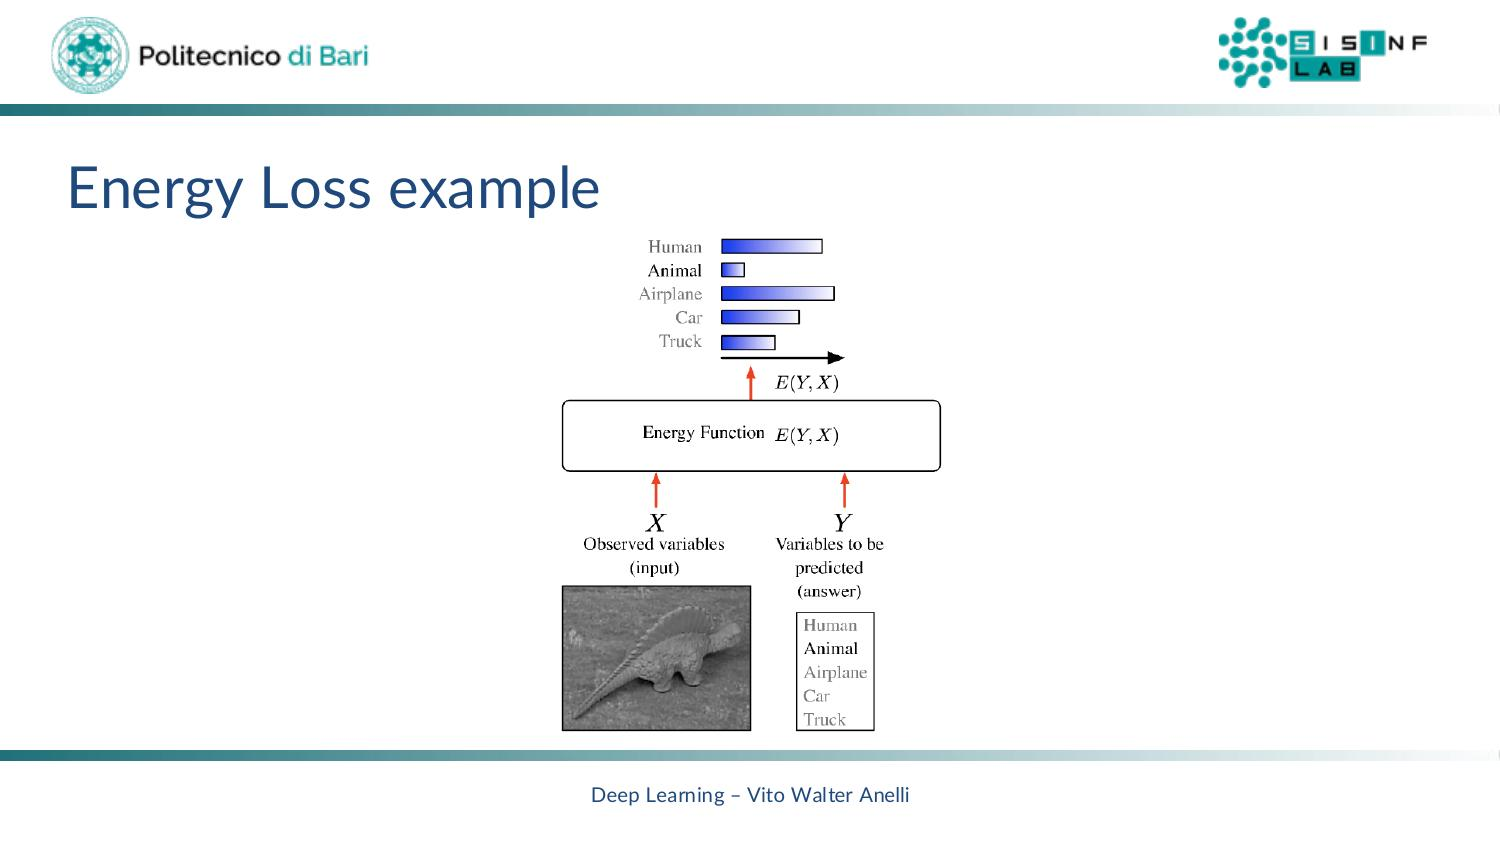
\includegraphics[width=0.85\linewidth]{figures/cf15_energy_loss_example.jpg}
  \caption{Esempio di funzione energia per un problema di classificazione.
           Dato un input $X$ (immagine di un animale) e le possibili
           etichette $Y$ \{Human, Animal, Airplane, Car, Truck\}, la
           funzione energia $E(Y,X)$ restituisce uno scalare per ogni coppia:
           un valore basso indica alta compatibilità tra $X$ e $Y$.}
  \label{fig:ebm-energy-loss-example}
\end{figure}

\subsection{Confronto con i Modelli Feed-Forward}
\label{subsec:ebm-vs-ff}

Un modello \textbf{feed-forward} è una funzione esplicita $\mathbf{y} =
G(\mathbf{x})$: ad ogni input corrisponde un unico output deterministico.
Un \textbf{EBM} è invece una funzione implicita che cattura la
dipendenza tra $\mathbf{x}$ e $\mathbf{y}$ tramite $F(\mathbf{x},
\mathbf{y})$. La differenza cruciale è che più valori di $\mathbf{y}$
possono essere compatibili con un singolo $\mathbf{x}$, corrispondendo
a minimi distinti della superficie energetica.

Perché la funzione $F$ sia utilizzabile con algoritmi di inferenza basati
su gradiente, essa deve essere \emph{liscia} e \emph{differenziabile}
rispetto a $\mathbf{y}$ (quando $\mathbf{y}$ è continuo). La superficie
energia deve presentare bassa energia in prossimità dei punti del dataset
e alta energia altrove.

\begin{figure}[H]
  \centering
  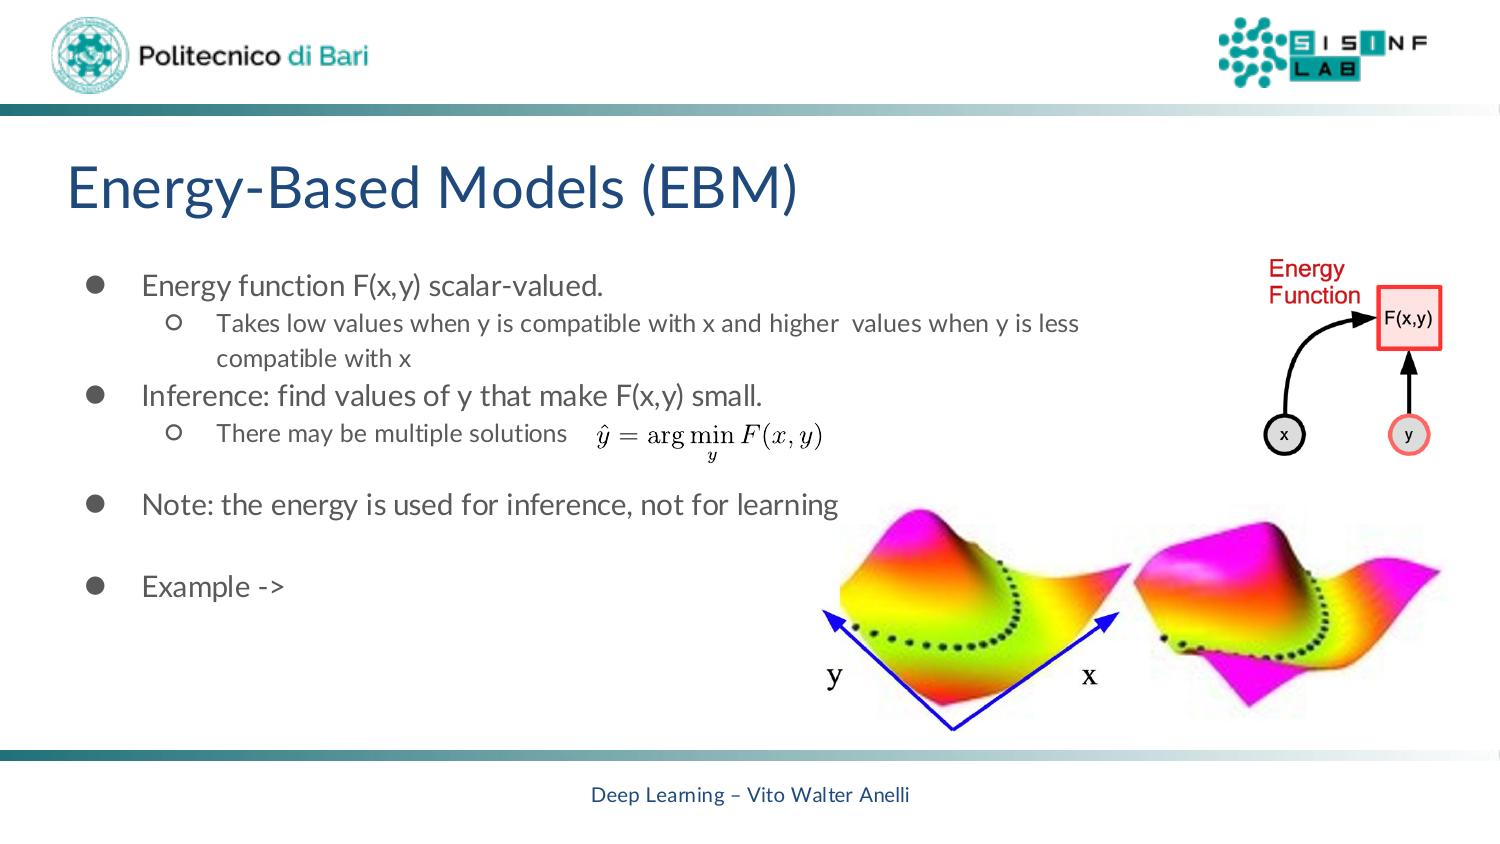
\includegraphics[width=0.85\linewidth]{figures/cf15_ebm_inference.jpg}
  \caption{Superficie energia $F(x,y)$ in funzione delle variabili $x$
           e $y$. La curva tratteggiata indica i punti del training set:
           la rete apprende a collocare i minimi della superficie in
           corrispondenza dei dati osservati. L'inferenza corrisponde a
           discendere il gradiente lungo la dimensione $y$.}
  \label{fig:ebm-inference}
\end{figure}

\subsection{Superfici Energetiche: Buon e Cattivo Addestramento}
\label{subsec:ebm-surfaces}

Un addestramento corretto modella la superficie energetica in modo che
presenti valli nette in prossimità dei dati di training e colline altrove.
Al contrario, un addestramento difettoso può portare alla cosiddetta
\textbf{soluzione collassata}: il modello ignora l'input e produce output
identici, generando una superficie piatta con energia prossima a zero
ovunque. Questo comportamento degenere è il principale rischio dei metodi
privi di un meccanismo esplicito di separazione delle regioni a bassa
energia.

\begin{figure}[H]
  \centering
  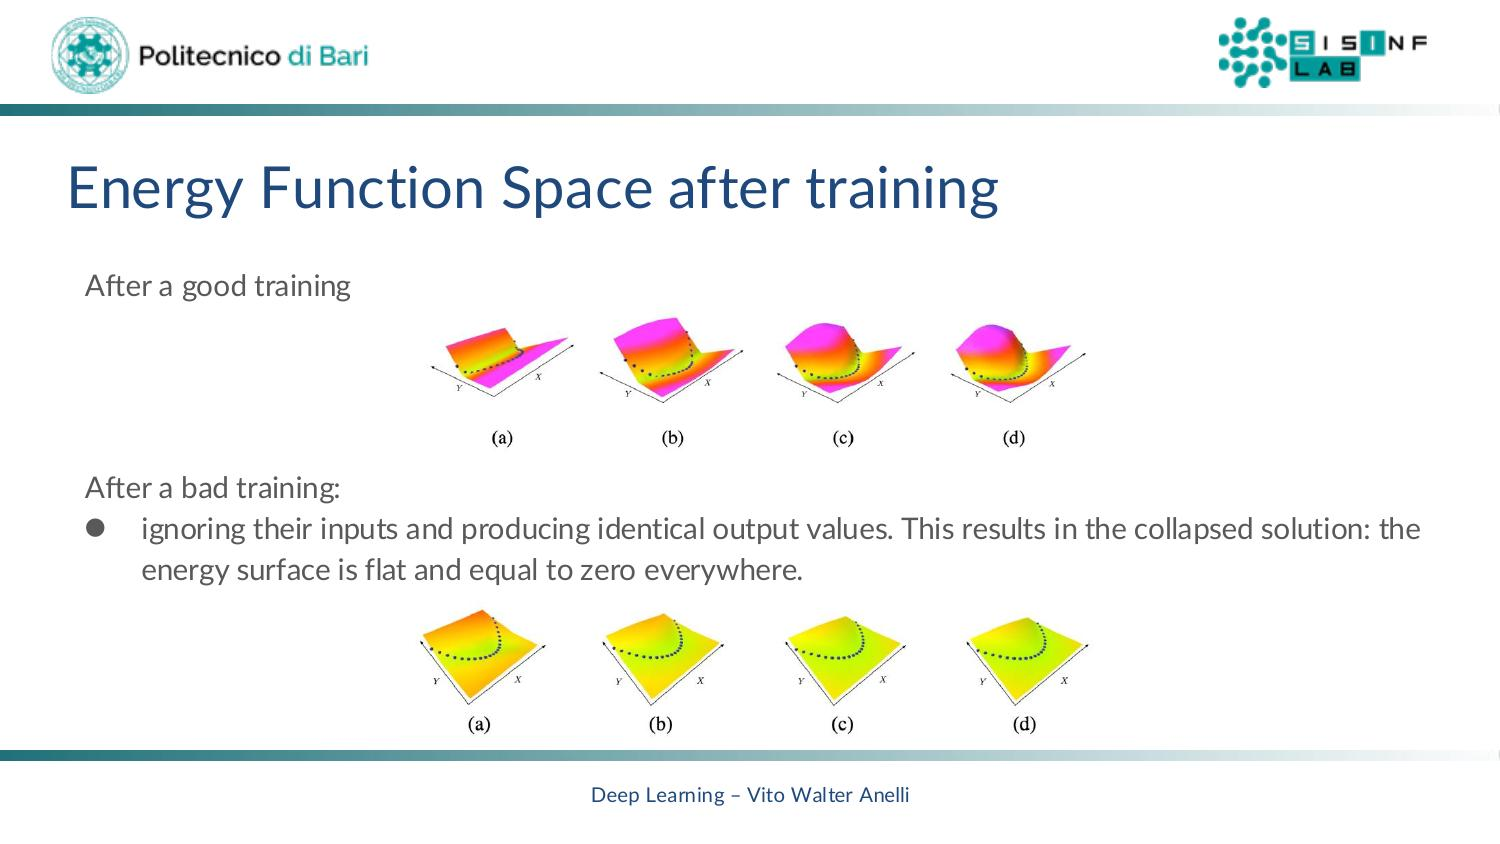
\includegraphics[width=0.88\linewidth]{figures/cf15_energy_surface_training.jpg}
  \caption{Confronto tra superfici energia dopo un buon addestramento
           (riga superiore) e un cattivo addestramento (riga inferiore).
           Nel caso degenere la superficie è piatta (energia costante),
           impedendo qualsiasi discriminazione tra output compatibili e
           incompatibili.}
  \label{fig:ebm-surfaces}
\end{figure}

%------------------------------------------------------------
\section{Architetture EBM per la Predizione Multimodale}
\label{sec:ebm-architectures}

Per gestire distribuzioni multimodali sull'output esistono due famiglie
principali di architetture: i \textbf{joint embedding architectures} e
i \textbf{latent variable models}.

\subsection{Joint Embedding}
\label{subsec:joint-embedding}

Nell'architettura a \textbf{joint embedding}, due rami encoder ($\text{Pred}(x)$
e $\text{Pred}(y)$) proiettano input e output nello stesso spazio delle
feature, producendo le rappresentazioni $\mathbf{h}$ e $\mathbf{h}'$.
La funzione energia è definita come una misura di distanza in questo spazio:
\begin{equation}
  F(\mathbf{x}, \mathbf{y}) = C\bigl(\mathbf{h},\, \mathbf{h}'\bigr),
\end{equation}
dove $C(\cdot, \cdot)$ è tipicamente la distanza euclidea o coseno.
Le multiple predizioni compatibili sono ottenute tramite invarianza alle
features piuttosto che tramite ricostruzione a livello di pixel.

Vantaggi principali:
\begin{itemize}
  \item Nessuna ricostruzione pixel-level, computazionalmente onerosa.
  \item Naturalmente invariante a distorsioni semanticamente irrilevanti
        (illuminazione, prospettiva, occlusioni parziali).
\end{itemize}

Esempi di successo per il riconoscimento di immagini includono
DeepFace~\citep{taigman2014deepface}, PIRL, MoCo e SimCLR.

\subsection{Modelli a Variabili Latenti}
\label{subsec:latent-variable-ebm}

Nei \textbf{modelli a variabili latenti} (LV-EBM), una variabile latente
$\mathbf{z}$ parametrizza l'insieme delle predizioni compatibili con
l'input. Idealmente, $\mathbf{z}$ cattura fattori esplicativi
\emph{indipendenti} della variabilità dell'output. L'architettura è
composta da:

\begin{description}
  \item[$\text{Pred}(x)$] Encoder che produce la rappresentazione
        $\mathbf{h}$ a partire dall'osservazione $\mathbf{x}$.
  \item[$\text{Dec}(\mathbf{z}, \mathbf{h})$] Decoder che genera la
        predizione $\bar{\mathbf{y}}$ combinando $\mathbf{h}$ con la
        variabile latente $\mathbf{z}$.
\end{description}

È critico che la \textbf{capacità informativa} di $\mathbf{z}$ sia
limitata: se $\mathbf{z}$ può memorizzare tutta l'informazione
sull'output, il modello potrebbe ricostruire perfettamente qualsiasi
$\mathbf{y}$ indipendentemente da $\mathbf{x}$, collassando sulla
soluzione banale con superficie piatta.

\paragraph{Esempi applicativi.}
Le variabili latenti sono particolarmente utili quando l'inferenza richiede
informazione ausiliaria non osservata. Per esempio, riconoscere una parola
manoscritta è facilitato dalla conoscenza implicita della posizione dei
caratteri; per il riconoscimento del parlato, conoscere la posizione dei
fonemi e delle parole nell'audio semplifica enormemente il task.

\subsection{LV-EBM Condizionale con Regolarizzazione}
\label{subsec:conditional-lv-ebm}

Per evitare la soluzione collassata, il modello condizionale adotta un
\textbf{regolarizzatore} $R(\mathbf{z})$ che penalizza la capacità di
$\mathbf{z}$. La funzione energia diventa:
\begin{equation}
  E(\mathbf{x}, \mathbf{y}, \mathbf{z})
  = C\!\bigl(\mathbf{y},\; \text{Dec}(\text{Pred}(\mathbf{x}),\, \mathbf{z})\bigr)
  + \lambda\, R(\mathbf{z}).
  \label{eq:conditional-lv-ebm}
\end{equation}

Esempi di regolarizzatori efficaci:
\begin{itemize}
  \item \textbf{Dimensione effettiva} \citep{li2020rethinking}: penalizza
        il rango effettivo della rappresentazione latente.
  \item \textbf{Quantizzazione/discretizzazione}: limita $\mathbf{z}$ a
        un insieme discreto di valori (come nei VQ-VAE).
  \item \textbf{Norma $\ell_0$}: minimizza il numero di componenti non nulle
        di $\mathbf{z}$.
  \item \textbf{Norma $\ell_1$} con normalizzazione del decoder.
  \item \textbf{Inibizione laterale}: promuove la competizione tra unità
        latenti.
  \item \textbf{Aggiunta di rumore} con vincolo sulla norma $\ell_2$
        di $\mathbf{z}$ (come nei VAE~\citep{kingma2013vae}).
\end{itemize}

%------------------------------------------------------------
\section{Addestramento degli EBM}
\label{sec:ebm-training}

L'obiettivo dell'addestramento è plasmare la funzione
$F_\theta(\mathbf{x},\mathbf{y})$, parametrizzata da $\theta$, in modo
che:
\begin{equation}
  F_\theta\!\bigl(\mathbf{x}^{(i)}, \mathbf{y}^{(i)}\bigr)
  <
  F_\theta\!\bigl(\mathbf{x}^{(i)}, \mathbf{y}\bigr)
  \quad \forall\, \mathbf{y} \neq \mathbf{y}^{(i)},
\end{equation}
mantenendo al contempo $F$ \emph{liscia}. I metodi di apprendimento si
dividono in due grandi categorie.

\begin{figure}[H]
  \centering
  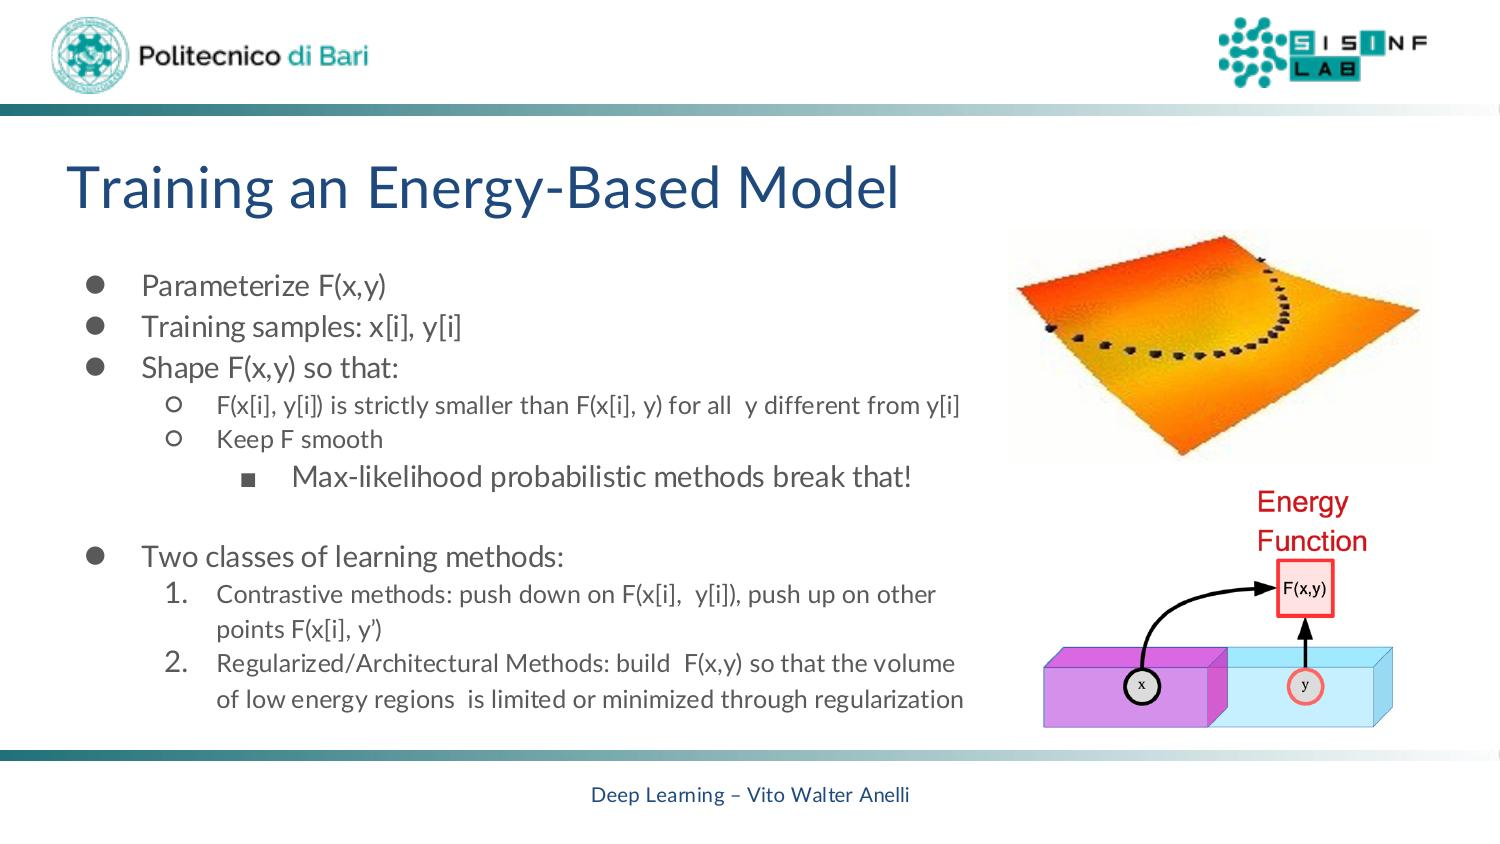
\includegraphics[width=0.75\linewidth]{figures/cf15_training_ebm.jpg}
  \caption{Configurazione per l'addestramento di un EBM. La funzione
           energia $F(\mathbf{x},\mathbf{y})$ viene parametrizzata e
           addestrata a collocare i minimi in corrispondenza dei
           campioni del training set.}
  \label{fig:ebm-training}
\end{figure}

\subsection{Metodi Contrastivi}
\label{subsec:contrastive-methods}

I \textbf{metodi contrastivi} operano con una strategia \emph{push-down /
push-up}: abbassano l'energia sui punti del training set
$(\mathbf{x}^{(i)}, \mathbf{y}^{(i)})$ e la alzano su punti alternativi
$(\mathbf{x}^{(i)}, \mathbf{y}')$ denominati \emph{campioni negativi}
o \emph{contrastivi}.

\begin{figure}[H]
  \centering
  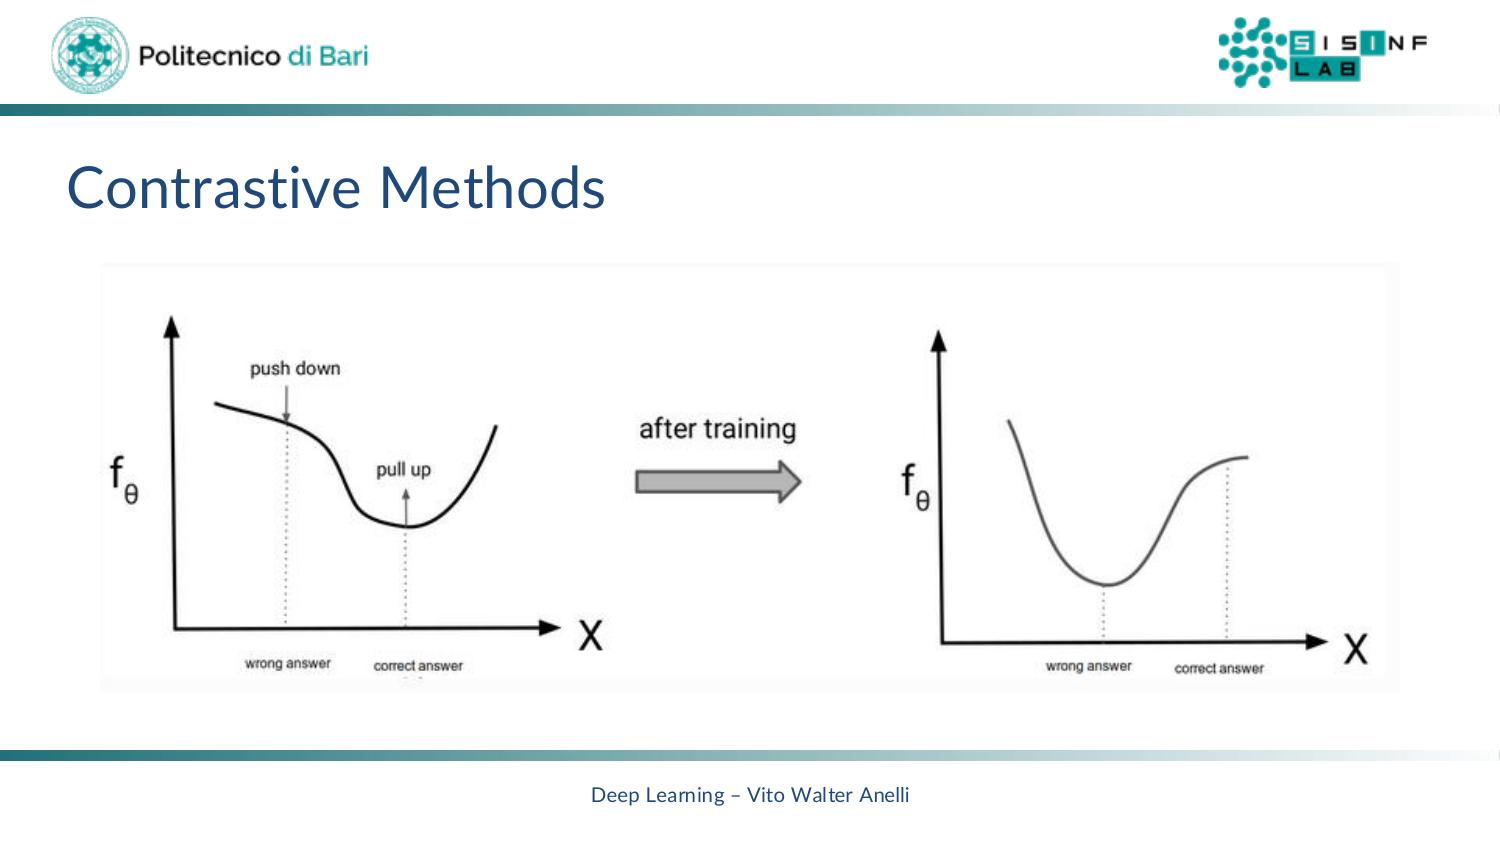
\includegraphics[width=0.80\linewidth]{figures/cf15_contrastive_push_down.jpg}
  \caption{Dinamica dei metodi contrastivi. A sinistra: lo stato iniziale
           prima dell'addestramento con frecce che indicano le direzioni
           di push-down (campione corretto) e push-up (campione errato).
           A destra: la superficie energia dopo l'addestramento, con il
           minimo ben collocato in corrispondenza dell'output corretto.}
  \label{fig:ebm-contrastive-pushdown}
\end{figure}

\paragraph{Interpretazione probabilistica.}
L'energia può essere interpretata come log-densità non normalizzata
(negativa) tramite la \textbf{distribuzione di Gibbs}:
\begin{equation}
  P(\mathbf{y} \mid \mathbf{x}) =
  \frac{\exp\!\bigl[-\beta F(\mathbf{x}, \mathbf{y})\bigr]}
       {\displaystyle\int_{\mathbf{y}'} \exp\!\bigl[-\beta F(\mathbf{x}, \mathbf{y}')\bigr]\, \mathrm{d}\mathbf{y}'},
  \label{eq:gibbs}
\end{equation}
dove $\beta > 0$ è un parametro analogo alla temperatura inversa. Il
denominatore è la \textbf{funzione di partizione} $Z(\mathbf{x})$, spesso
intrattabile per spazi continui ad alta dimensione: questo è il motivo
principale per cui si preferisce evitare l'approccio probabilistico quando
non strettamente necessario.

\paragraph{Massima verosimiglianza.}
Massimizzare $P(\mathbf{y}^{(i)} \mid \mathbf{x}^{(i)})$ equivale a
minimizzare la \emph{negative log-likelihood} (NLL):
\begin{equation}
  \mathcal{L}(\mathbf{y},\mathbf{w})
  = E(\mathbf{y}, \mathbf{w})
  + \frac{1}{\beta}\log\!\int_{\mathbf{y}'} e^{-\beta E(\mathbf{y}',\mathbf{w})},
  \label{eq:nll-loss}
\end{equation}
dove il primo termine va minimizzato (abbassare l'energia sul campione
corretto) e il secondo va massimizzato (alzare l'energia ovunque altrove).

\paragraph{Problema con la massima verosimiglianza.}
La NLL tende a creare un canyon infinitamente profondo e stretto attorno
alla varietà dei dati: vuole massimizzare la differenza di energia tra
i punti del dataset e quelli appena fuori di esso. Questo rende la
superficie non liscia e incompatibile con l'inferenza basata su gradiente.
È pertanto necessario regolarizzare la funzione di perdita (ad esempio con
la distanza di Wasserstein nelle WGAN) per recuperare la proprietà di
smoothness.

\begin{figure}[H]
  \centering
  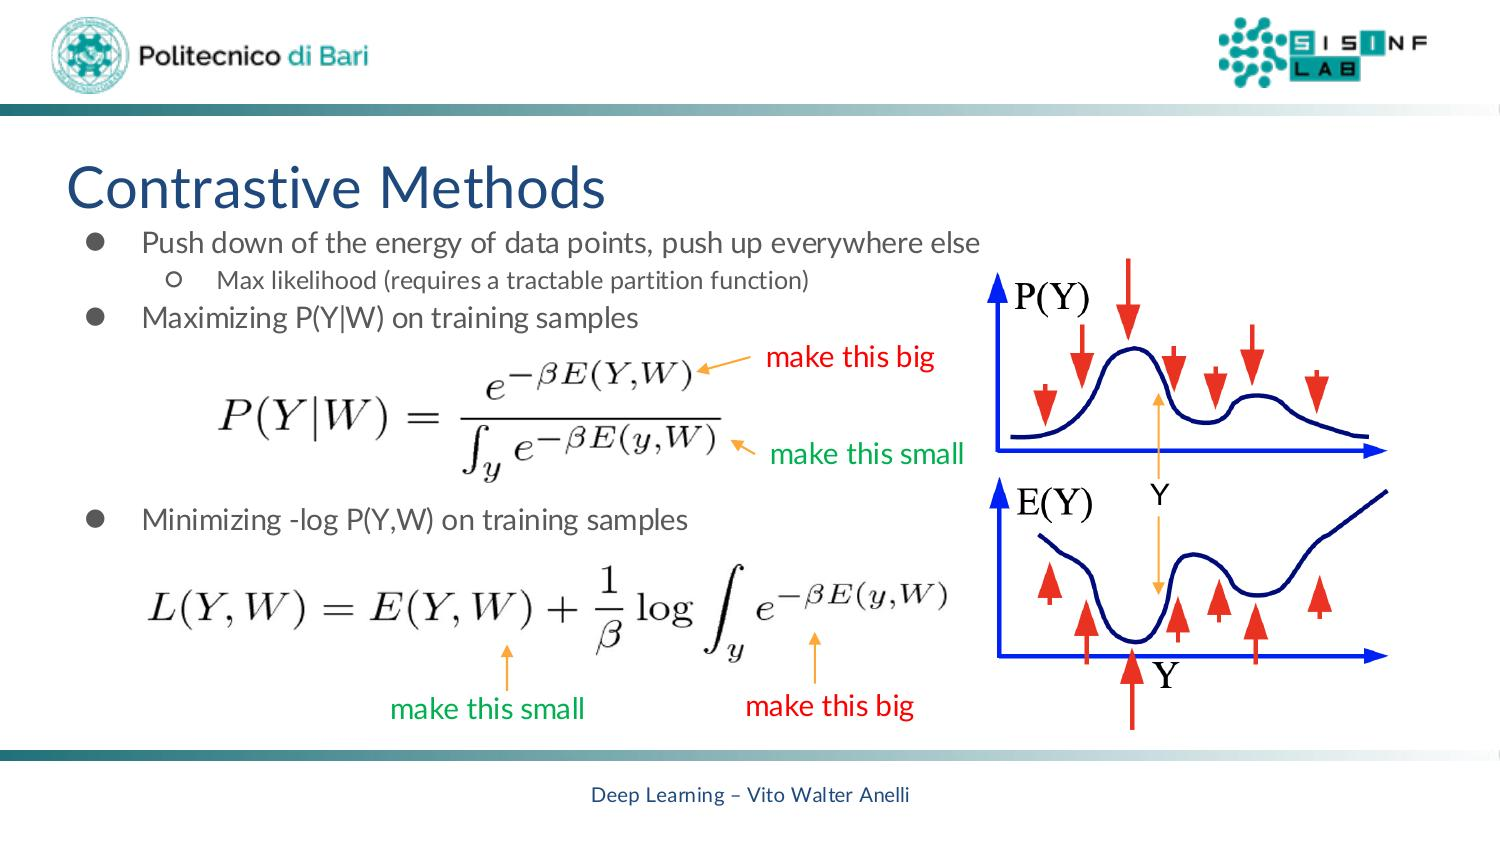
\includegraphics[width=0.85\linewidth]{figures/cf15_contrastive_methods.jpg}
  \caption{Metodi contrastivi in pratica: la probabilità $P(Y|W)$ viene
           massimizzata (riga superiore) portando a un abbassamento
           dell'energia sui campioni corretti e a un innalzamento
           ovunque altrove (riga inferiore).}
  \label{fig:ebm-contrastive}
\end{figure}

\subsection{Addestramento con MCMC}
\label{subsec:mcmc-training}

L'algoritmo pratico per l'addestramento contrastivo, proposto in
\citet{du2019implicit}, sfrutta un buffer di campioni e la
\emph{Langevin dynamics} (una forma di MCMC) per generare campioni negativi:

\begin{enumerate}
  \item Campionare un esempio reale $\mathbf{x}^+_i \sim p_\mathcal{D}$.
  \item Estrarre un campione iniziale dal buffer $B$ con probabilità 95\%,
        o da $\mathcal{U}(-1,1)$ con probabilità 5\%.
  \item Per $k = 1,\ldots,K$ passi, aggiornare il campione con la
        \textbf{Langevin dynamics}:
        \begin{equation}
          \tilde{\mathbf{x}}^k \leftarrow \tilde{\mathbf{x}}^{k-1}
          - \eta\, \nabla_{\mathbf{x}} E_\theta(\tilde{\mathbf{x}}^{k-1})
          + \omega,
          \quad \omega \sim \mathcal{N}(0,\sigma),
        \end{equation}
        ottenendo il campione negativo $\mathbf{x}^- = \tilde{\mathbf{x}}^K$.
  \item Calcolare la \textbf{contrastive divergence loss}:
        \begin{equation}
          \mathcal{L}_{CD} = \frac{1}{N}\sum_i
          E_\theta(\mathbf{x}^+_i) - E_\theta(\mathbf{x}^-_i),
        \end{equation}
        e la \textbf{regularization loss}:
        \begin{equation}
          \mathcal{L}_{RG} = \frac{1}{N}\sum_i
          \bigl[E_\theta(\mathbf{x}^+_i)\bigr]^2
          + \bigl[E_\theta(\mathbf{x}^-_i)\bigr]^2.
        \end{equation}
  \item Aggiornare i parametri con SGD/Adam su
        $\nabla_\theta(\mathcal{L}_{CD} + \alpha\,\mathcal{L}_{RG})$.
  \item Aggiungere $\mathbf{x}^-$ al buffer $B$.
\end{enumerate}

\subsection{Metodi Regolarizzati e Architetturali}
\label{subsec:regularized-methods}

I \textbf{metodi regolarizzati} non richiedono campioni negativi espliciti:
costruiscono $F(\mathbf{x},\mathbf{y})$ in modo che il volume delle regioni
a bassa energia sia intrinsecamente limitato tramite la struttura
dell'architettura o un termine di regolarizzazione.
Questi metodi includono autoencoder, VAE, normalizing flows e le architetture
a joint embedding non contrastive discusse nella Sezione~\ref{sec:ssl}.

%------------------------------------------------------------
\section{Funzioni di Perdita per EBM}
\label{sec:ebm-loss-functions}

La scelta della funzione di perdita è cruciale: le perdite efficaci
devono avere un \textbf{margine non nullo}, ovvero devono garantire che
l'energia del campione corretto sia strettamente inferiore a quella dei
campioni negativi di almeno una quantità $m > 0$.

\begin{figure}[H]
  \centering
  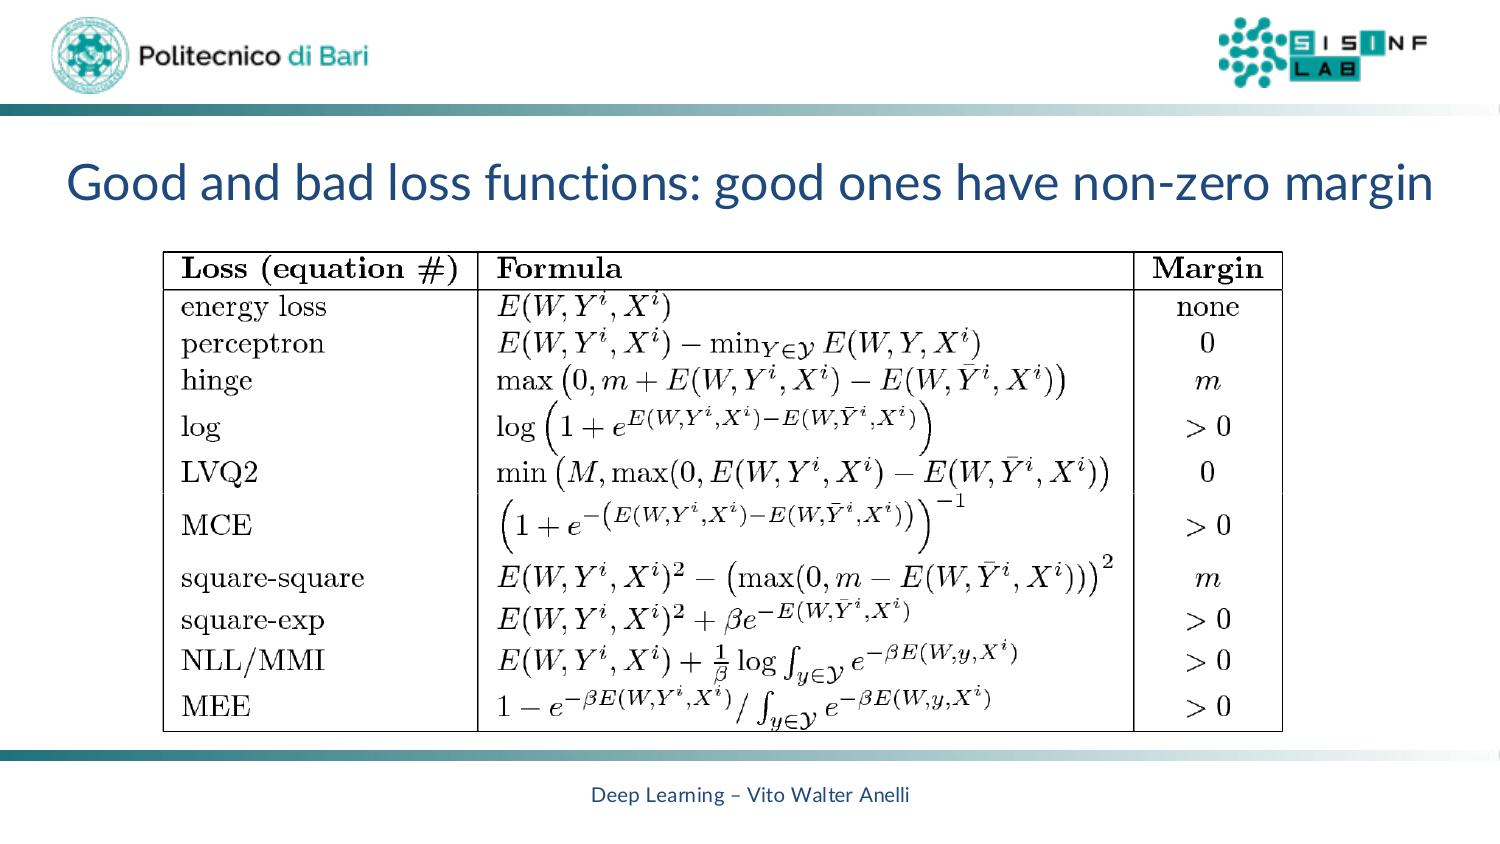
\includegraphics[width=0.90\linewidth]{figures/cf15_loss_functions_table.jpg}
  \caption{Riepilogo delle principali funzioni di perdita per EBM.
           Le perdite con margine non nullo (hinge, square-square,
           MCE, NLL/MMI, MEE, square-exp) sono in genere preferibili
           alla perdita energetica pura e alla perdita percettrone,
           che hanno margine nullo o assente.}
  \label{fig:ebm-loss-functions}
\end{figure}

Le perdite più comuni sono riportate in Tabella~\ref{tab:ebm-losses}.

\begin{table}[H]
  \centering
  \caption{Principali funzioni di perdita per EBM, con relativo margine.
           $E^+\!=\!E(W,Y^i,X^i)$ è l'energia del campione corretto,
           $E^-\!=\!E(W,\bar{Y}^i,X^i)$ è l'energia del campione
           negativo più favorevole.}
  \label{tab:ebm-losses}
  \small
  \begin{tabular}{lll}
    \toprule
    \textbf{Perdita} & \textbf{Formula} & \textbf{Margine} \\
    \midrule
    Energy loss    & $E^+$                                              & nessuno \\
    Perceptron     & $E^+ - \min_{Y\in\mathcal{Y}} E(W,Y,X^i)$          & 0 \\
    Hinge          & $\max(0,\; m + E^+ - E^-)$                         & $m$ \\
    Log            & $\log\!\left(1 + e^{E^+ - E^-}\right)$             & $>0$ \\
    LVQ2           & $\min\!\left(M,\;\max(0,\;E^+ - E^-)\right)$       & 0 \\
    MCE            & $\left(1 + e^{-(E^+ - E^-)}\right)^{-1}$           & $>0$ \\
    Square-square  & $(E^+)^2 - \bigl(\max(0,\;m - E^-)\bigr)^2$        & $m$ \\
    Square-exp     & $(E^+)^2 + \beta\,e^{-E^-}$                        & $>0$ \\
    NLL/MMI        & $E^+ + \frac{1}{\beta}\log\!\int e^{-\beta E}$      & $>0$ \\
    MEE            & $1 - e^{-\beta E^+}\!/\!\int e^{-\beta E}$          & $>0$ \\
    \bottomrule
  \end{tabular}
\end{table}

%------------------------------------------------------------
\section{Joint Embedding Contrastivo}
\label{sec:contrastive-joint-embedding}

Il \textbf{joint embedding contrastivo} combina la struttura a doppio
encoder con la strategia push-down/push-up. Le coppie di campioni sono
di due tipi:

\begin{description}
  \item[Coppia positiva] ($\mathbf{x}$ e $\mathbf{y}$ semanticamente
        equivalenti, ad esempio due viste della stessa immagine): la
        funzione energia $F$ deve essere \emph{piccola}.
  \item[Coppia negativa] ($\mathbf{x}$ e $\mathbf{y}$ semanticamente
        diversi): la funzione energia $F$ deve essere \emph{grande}.
\end{description}

\begin{figure}[H]
  \centering
  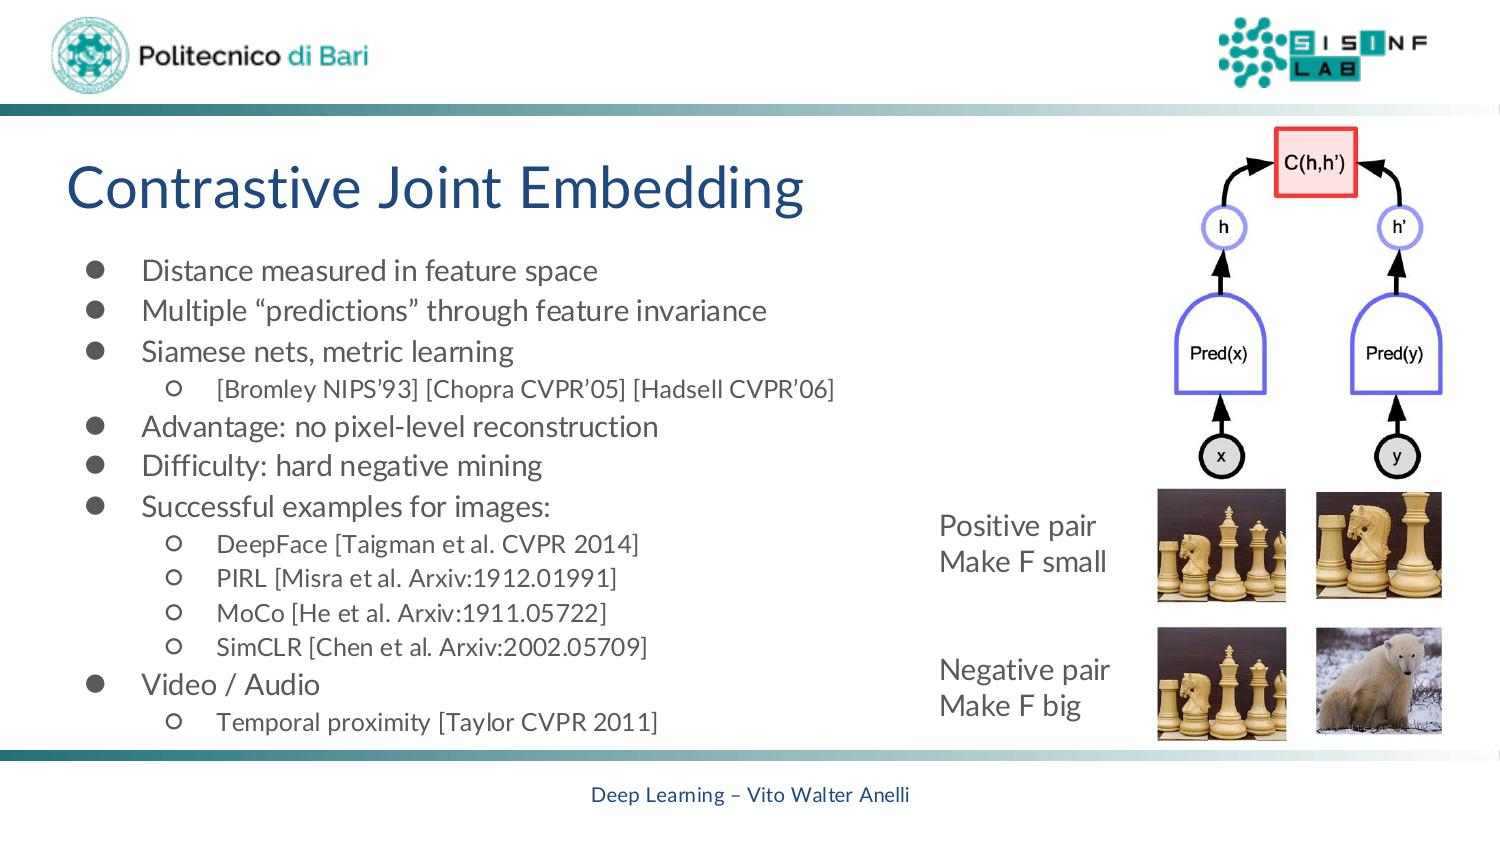
\includegraphics[width=0.85\linewidth]{figures/cf15_contrastive_joint_embedding.jpg}
  \caption{Architettura del joint embedding contrastivo. Due encoder
           $\text{Pred}(x)$ e $\text{Pred}(y)$ proiettano le coppie di
           input nello stesso spazio di feature. La distanza $C(\mathbf{h},
           \mathbf{h}')$ viene minimizzata per le coppie positive (stessa
           scena, diverse prospettive) e massimizzata per le coppie
           negative (scena diversa). Il vantaggio principale è l'assenza
           di ricostruzione pixel-level; la difficoltà principale è il
           \emph{hard negative mining}.}
  \label{fig:contrastive-joint-embedding}
\end{figure}

La principale difficoltà pratica è il \textbf{hard negative mining}: è
necessario identificare campioni negativi sufficientemente informativi
(quelli con bassa energia ma etichetta errata), poiché campioni negativi
facili non forniscono gradiente utile all'addestramento.

\subsection{Joint Embedding Non Contrastivo}
\label{subsec:non-contrastive-embedding}

Per eliminare la necessità di campioni negativi espliciti, i metodi
non contrastivi come \textbf{BYOL}~\citep{grill2020byol}
(\emph{Bootstrap Your Own Latent}, Google DeepMind) e
\textbf{SimSiam}~\citep{chen2021simsiam} adottano una rete siamese
con pesi leggermente diversi tra i due rami. Il ramo \emph{target}
utilizza una media mobile esponenziale (\emph{exponential moving average})
dei pesi del ramo \emph{online}. Questo meccanismo di asimmetria
costituisce un regolarizzatore implicito che impedisce il collasso, senza
richiedere coppie negative.

%------------------------------------------------------------
\section{Self-Supervised Learning}
\label{sec:ssl}

Il \textbf{self-supervised learning} (SSL) risponde alla domanda su come
gli esseri umani e gli animali apprendono a modellare il mondo con
pochissima supervisione esplicita. Nella fase neonatale, l'apprendimento
avviene in larga misura per osservazione: si accumula una quantità
enorme di conoscenza contestuale sulla struttura fisica del mondo
(permanenza degli oggetti, solidity, gravità, inerzia) che costituisce
la base del senso comune.

Nel SSL la \textbf{supervisione è generata autonomamente dai dati stessi}:
si mascherano o corrompono parti dell'input e si addestra il modello a
ricostruirle. Formalmente:
\begin{center}
  \emph{``Predire ogni parte dell'input a partire da tutte le altre.''}
\end{center}

Questo include: predire il futuro dal passato in sequenze temporali,
predire le regioni occultate di un'immagine, completare token mancanti
in una sequenza testuale (come in BERT e GPT).

\subsection{SSL come Riempimento dei Vuoti}
\label{subsec:ssl-fill-blanks}

Il SSL può essere visto come una forma di \emph{riempimento dei vuoti}
(\emph{filling in the blanks}): data una finestra di input, si nasconde
arbitrariamente una porzione (nel tempo, nello spazio, o in entrambi) e
si chiede al modello di predirla. La ricostruzione è un caso speciale di
SSL in cui qualsiasi parte dell'input può essere nota o ignota.

\paragraph{Wav2Vec 2.0.}
Un esempio paradigmatico di SSL applicato al parlato è
\textbf{Wav2Vec 2.0}~\citep{baevski2020wav2vec}: preaddestrato su
960 ore di parlato non etichettato, richiede solo 10 minuti di dati
etichettati per eguagliare le prestazioni del precedente stato dell'arte
che usava 100 ore di etichette. Questo risultato illustra l'efficacia
delle rappresentazioni apprese in modo self-supervised.

\paragraph{Modelli linguistici moderni.}
Nel dominio del testo, i modelli di linguaggio basati su SSL (GPT, BERT,
XLNet, RoBERTa, ALBERT) hanno raggiunto e superato le prestazioni umane
su benchmark di comprensione del testo come il RACE challenge (lettura
tipo SAT), con ALBERT che raggiunge un'accuratezza di 89.4 a fronte di
una baseline umana di circa 95.0 e del precedente SOTA a 83.2.

%------------------------------------------------------------
\section{Connessioni con i Modelli Generativi}
\label{sec:ebm-generative}

\subsection{Relazione con i VAE}
\label{subsec:ebm-vae}

I \textbf{Variational Autoencoders} (VAE) sono un caso speciale di
LV-EBM condizionale in cui il regolarizzatore è la divergenza KL tra la
distribuzione posteriore di $\mathbf{z}$ e una gaussiana standard:
$R(\mathbf{z}) = D_\mathrm{KL}\!\bigl(q(\mathbf{z}|\mathbf{x})
\;\|\; \mathcal{N}(0,I)\bigr)$.
Il rumore aggiunto a $\mathbf{z}$ durante l'addestramento, combinato con
il vincolo sulla norma $\ell_2$, costituisce il meccanismo che limita la
capacità informativa della variabile latente.

\subsection{Confronto con i Metodi Contrastivi e i VAE}
\label{subsec:cd-vs-vae}

\begin{table}[H]
  \centering
  \caption{Confronto tra metodi contrastivi e Variational Autoencoders
           come approcci alternativi per l'addestramento di EBM.}
  \label{tab:cd-vs-vae}
  \small
  \begin{tabular}{lll}
    \toprule
    \textbf{Aspetto}            & \textbf{Metodi Contrastivi}         & \textbf{VAE}                        \\
    \midrule
    Obiettivo principale        & Regolare un EBM                     & Generare dati e apprendere          \\
                                &                                     & una distribuzione esplicita         \\
    Strategia di addestramento  & MCMC per approssimazione            & Discesa del gradiente su ELBO       \\
    Tipo di distribuzione       & Implicita (non parametrica)         & Esplicita (es. gaussiana)           \\
    Efficienza di campionamento & Lenta (più iterazioni MCMC)         & Veloce (spazio latente              \\
                                &                                     & parametrizzato)                     \\
    \bottomrule
  \end{tabular}
\end{table}

%------------------------------------------------------------
\section{Architettura Pratica: ConvNet come EBM}
\label{sec:ebm-convnet}

Un EBM può essere implementato con qualsiasi architettura differenziabile.
Una scelta comune è una \textbf{rete convoluzionale feed-forward} (ConvNet)
che mappa il segnale di input a uno scalare (l'energia). L'architettura
si compone di strati convoluzionali interlacciati con strati di
sottocampionamento, terminando con uno o più strati fully-connected che
producono lo scalare di energia $F(\mathbf{x}, \mathbf{y})$.

Questa configurazione è efficiente poiché sfrutta la condivisione dei
parametri e la località delle connessioni, ed è completamente
differenziabile, consentendo sia l'inferenza per discesa del gradiente
sia l'addestramento tramite backpropagation.
